%  Typ dokumentu - článek, prezentace aj.
\documentclass[english]{article}

%  Nastaví vstupní a výstupní kódování znaků (encoding) a lokalizace
\usepackage[T1]{fontenc}
\usepackage[utf8]{inputenc}
\usepackage[english,czech]{babel}
\usepackage{icomma}

%  Formát papíru a odsazení od jeho okrajů
\usepackage[letterpaper]{geometry}
\geometry{verbose,tmargin=1.5cm,bmargin=2cm,lmargin=2cm,rmargin=2cm}

%  Umožňuje pracovat s grafikou
\usepackage{graphicx}
\usepackage{bigstrut}
\usepackage{epstopdf}

%  Automaticky odsadí i první paragraf v každé sekci
\usepackage{indentfirst}

%  Umožňuje rozdělovat obsah na více sloupců
\usepackage{multicol}
\usepackage{booktabs}

%  Umožňuje používat hypertextové odkazy, nastavuje jejich barvu a
%  vlastnosti
\usepackage[unicode]{hyperref}
\hypersetup{
colorlinks=true, citecolor=blue, filecolor=blue, linkcolor=blue,
urlcolor=blue
}

%  Umožnění odstranění italiky u jednotek
\newcommand{\unit}[1]{\mathrm{#1}}

%  Formátování stránek, empty = odstraní číslování
% \pagestyle{empty}

%  Řádkování
\linespread{1.2}

%  Lepší zobrazování matematiky (rozšíření sum o \limits atd.)
\everymath{\displaystyle}
\usepackage{amsmath, amsthm, amssymb}

% Umožní psát přes \mathbb{N/R/Q/..} množiny čísel
\usepackage{amssymb}

%  Velikost fontu matematických výrazů v dokumentu lze pro danou
% základního fontu dokumentu upravit pomocí:
% \DeclareMathSizes{X}{Y}{Z}{U} kde:
% X je velikost fontu v dokumentu, pro kterou se matematika upraví
% Y je standartní velikost fontu matematiky
% Z je velikost fontu zmenšených (vnořených výrazů)
% U je velikost fontu ještě více zmenšených (vnořených výrazů).
\DeclareMathSizes{10}{10.5}{9}{9}

%  Nastaví autora, název, datum, skupinu měření apod. (můj vlastní
% příkaz, umožní znovu-použití v dokumentu)
\newcommand{\Author}{David Roesel}
\newcommand{\Coauthor}{Tereza Schönfeldová}
\newcommand{\Institute}{FJFI ČVUT v Praze}
\newcommand{\Subject}{FYZIKÁLNÍ PRAKTIKUM II}
\newcommand{\Group}{7}
\newcommand{\Circle}{ZS 7}
\newcommand{\Title}{Úloha \#8  \\Mikrovlny}
\newcommand{\Date}{3.3.2014}

% Začátek dokumentu - Formátování na výstup
\begin{document}

% Interní proměnné, možno zobrazovat u prezentací, používají se při
% generování pomocí \titlepage apod.
\author{\Author}
\title{\Title}
\date{\Date}

%  Lokalizace některých názvů do češtiny
\renewcommand{\figurename}{Obr.}
\renewcommand{\tablename}{Tab.}
\renewcommand{\refname}{Reference}

% --- Hlavička dokumentu -----------------------------------------------

\setlength{\parindent}{0cm}
\begin{multicols}{2}
\textbf{\Subject \\
        \Institute \\[0.1cm]
%\large  \Title \\[0.5cm]
\Title \\[0.5cm]
}
\begin{tabular}{rlrl}
\large Datum měření: & \Date & \large Skupina: & \Group \\
\large Jméno: & \Author & \large Kroužek:  & \Circle\\
\large Spolupracovala: & \Coauthor &\large Klasifikace:\\
\end{tabular}

\begin{flushright}
\includegraphics[scale=0.28]{../../_meta/fjfi_standart.pdf}
\hspace{0.2cm}
\includegraphics[scale=0.28]{../../_meta/cvut_standart.pdf}
\end{flushright}
\end{multicols}
\hrule
\vspace{0.5cm}

% ----------------------------------------------------------------------


% --- Tělo dokumentu ---------------------------------------------------
\setlength{\parindent}{0.5cm}
\section{Pracovní úkoly}
	  \begin{enumerate}
			\item Ověřte, že pole před zářičem je lineárně polarizované a určete směr polarizace. Ověřte Malusův zákon pro danou polarizační mřížku. Sestrojte dva grafy závislosti přijímaného napětí na úhlu pootočení polarizační mřížky nejprve pro sondu vertikálně a potom horizontálně.
			\item Proměřte rozložení elektromagnetického pole v rovině před zářičem a zobrazte jeho prostorový graf v programu Mathematica. Do protokolu zpracujte podélné a příčné rozložení pole (nezávislou veličinou budou souřadnice a závislou velikost napětí).
			\item Demonstrujte a proměřte stojaté vlnění. Z rozložení pole určete vlnovou délku. V druhé části pokusu vložte dielektrickou desku do pole stojaté vlny a pomocí vztahů odvozených v postupu stanovte index lomu dielektrické desky.
			\item Ověřte kvazioptické chování mikrovln -- difrakce na hraně, štěrbině a překážce, zákon lomu a fokusace čočkou. Spočítejte vlnovou délku z grafu vlnění na štěrbině a index lomu cukru pomocí ohniskové vzdálenosti čočky. Sestrojte příslušné grafy.
			\item Ověřte šíření mikrovln pomocí Lecherova vedení a vlnovodu. Ověřte, že podél Lecherova vedení se šíří stojatá vlna a určete z ní vlnovou délku.
	  \end{enumerate}

\section{Vypracování}

	\subsection{Použité přístroje}
	 Sonda elektrického pole, Gunnův oscilátor, trychtýřovitý nástavec, USB link PASCO, osobní počítač, program Data Studio, kartonová souřadnicová síť, otočná polarizační mřížka, sonda na detekci elektrického pole,  laboratorní stojan s nástavcem, držáky na desky, kovové desky, dielektrická deska PVC, pravítko, dutý půlválec, zdroj napětí se zesilovačem, cukr, konvexní čočka obsahující cukr, kovová cihla, kovový vlnovod, papírový úhloměr, kabely, kovové měřítko, Lecherovo vedení s kovovou spojkou.
						
	\subsection{Teoretický úvod}
		\subsubsection{Mikrovlnné záření}
				Jedná se o elektromagnetické záření s frekvencemi v rozsahu přibližně 300~MHz -- 300~GHz, kterému odpovídají vlnové délky $\approx$ 1~mm -- 1~m. Během měření jsme pracovali s tzv. \emph{Gunnovým oscilátorem}, který měl frekvenci přesně nastavenou na 9,4~GHz (což odpovídá vlnové délce 31,9~mm).
						
		\subsubsection{Gunnův oscilátor}
				Je znázorněný na Obr.~\ref{fig:gunnuv_oscilator_sonda} a skládá se z centrální části, která obsahuje Gunnovu diodu v obdélníkovém výřezu, kovové destičky vzadu a destičky s otvorem vepředu. Dohromady tím pádem tvoří dutinu, ve které se vytváří stojaté vlnění (z vln vysílaných Gunnovou diodou), které následně prochází otvorem do obdélníkového vlnovodu a lineárně polarizované ven. Vlnová délka vysílaného vlnění je tak zcela určena velikostí dutiny. 
				
				Pro detekci záření jsme používali přiloženou sondu (Obr.~\ref{fig:gunnuv_oscilator_sonda}). V našem případě šlo o tištěný spoj ve skleněné trubičce, jejíž vrchol plnil funkci dipólové antény. Směr polarizace signálu můžeme určit natáčením sondy a hledáním maximální intenzity signálu (při něm bude směr polarizace rovnoběžný se směrem sondy). 
				
				Funkci zdroje a zesilovače pro nás plní článek na Obr.~\ref{fig:zdroj_napeti_se_zesilovacem} a z jeho konstrukčního provedení má výstupní napětí zápornou hodnotu se zhruba stonásobným zesílením. Intenzitu pole v daném místě pro nás bude určovat absolutní hodnota odečítaného čísla.
							
		\subsubsection{Gaussovo rozdělení}
				K fitování píků využíváme funkci Gauss+konst. s předpisem
				\begin{equation}
						Gauss+konst.(x) = \frac{\alpha}{\sigma \sqrt{2\cdot \pi}} \cdot e^{-\frac{(x-\mu)^2}{2\sigma^2}} + \delta,
				\label{eq:gauss}
				\end{equation}
				kde $\alpha$ je amplituda, $\sigma$ strmost, $\mu$ posunutí a $\delta$ konstanta ve směru $y$.
			
	\subsection{Postup měření}
					Vzhledem k omezenému času na tak rozsáhlou úlohu jsme vůbec nezkoušeli zapojení s reproduktory a na všechny části postupu jsme tedy využívali standardního zapojení, které je na Obr.~\ref{fig:vychozi_nastaveni}, případně jsme ho lehce měnili v závislosti na konkrétní měřené úloze. Sonda převádí intenzitu na napětí a vzhledem k předpokládané přímé úměrnosti a našem zájmu na její změně (nikoliv absolutní hodnotě) jsme zaznamenávali právě hodnotu napětí. Tu jsme zobrazovali vždy v programu DataStudio a odtud opisovali. 
					
					Několik úkolů vyžadovalo zavedení kartézských souřadnic, což jsme učinili shodně s nákresem na Obr.~\ref{fig:soustava_souradnic}, tedy tak aby vertikální osa byla $y$, horizontální osa směřující přímo od vysílače $z$ a $x$ ve zbývajícím směru. Při všech experimentech jsme se snažili udržet stejnou výšku dipólové antény a středu nástavce vysílače. Konzistentně jsme se taktéž snažili volit natočení antény.
								
			\subsubsection{Polarizace}
					Sestavení úlohy je uvedeno na Obr.~\ref{fig:polarizace_malus}. Před vlastním měřením jsme se přesvědčili, že je záření z Gunnova oscilátoru opravdu lineárně polarizované otáčením sondy v rovině $x$-$y$ a sledováním změny intenzity v závislosti na otočení. 
					
					Následně jsme mezi zdroj a detektor umístili mikrovlnnou polarizační destičku, která propouští vždy jen záření polarizované v daném směru (záření je propouštěno vždy jen ve směru kolmém na proužky na destičce). 
								
					Snažili jsme se ověřit závislost danou Malusovým zákonem v podobě 
					\begin{equation}
					I(\theta) = I_0 \sin^4 \theta
					\label{eq:malus_vert}
					\end{equation}
					pro sondu umístěnou rovnoběžně s osou zářiče a
					\begin{equation}
					I(\theta) = 4 I_0 ( \sin \theta \cos \theta )^2
					\label{eq:malus_hori}
					\end{equation}
					pro sondu umístěnou kolmo na ni, kde úhel $\theta$ udává otočení polarizační mřížky při obou polohách sondy.
					
			\subsubsection{Rozložení pole}
					Podle přípravy jsme se snažili měřit pouze rozložení pole dalekého, tedy za (pro náš případ) definovanou hranicí 
					\begin{equation}
					r_0 = \frac{2 D_H^2}{\lambda_0},
					\end{equation}
					kde $D_H$ je největší rozměr antény a $\lambda_0$ vlnová délka. V našem případě bereme $r_0 = 100$~mm.
					
				    Vlastní měření jsme prováděli tak, že jsme před zdroj do vzdálenosti rovné $r_0$ umístili kartonovou souřadnou síť a ve všech jejích souřadnicích změřili intenzitu. 
					
			\subsubsection{Stojatá vlna}
					Stojatá vlna vzniká v momentu, kdy interferují dvě postupné vlny o opačném směru a stejné amplitudě. Pro určení vlnové délky $\lambda$ (a později také indexu lomu dielektrické desky) je třeba studovat vzdálenosti minim a maxim této vlny, která jsou od sebe vzdálena přesně $\lambda/2$. V přípravě je uvedena správná vzdálenost kovové desky od zářiče jako 200~mm, ale při této vzdálenosti dochází v okolí maxim k přehlcení detektoru a je tak velmi obtížné je obstojně určit. Proto jsme tuto vzdálenost volili dvakrát delší.
					
					V závislosti na vzdálenosti sondy od desky podél osy $z$ jsme měřili intenzitu a hledali minima a maxima. Jedno z nich jsme si vybrali a pokusili se ho znovu najít po vložení dielektrické desky mezi sondu a odraznou kovovou desku. Z tohoto posunutí je možné spočítat podle vzorce
					\begin{equation}
					n = \frac{z_2 - z_1}{d} + 1,
					\label{eq:index_lomu}
					\end{equation}
					index lomu dielektrické desky $n$, přičemž $z_1$ a $z_2$ jsou polohy maxima před a po vložení dielektrické desky a $d$ její tloušťka (vztah platí pro index lomu vzduchu $n_1=1$). Schématicky (ač ne zcela korektně, viz Diskuse) je posunutí minima znázorněno na Obr.~\ref{fig:index_lomu_desky}.
					
			\subsubsection{Ohyb na hraně}
					Aparaturu jsme sestavili dle nákresu na Obr.~\ref{fig:ohyb_na_hrane} a měřili závislost napětí na souřadnici $x$ od $-80$~mm do $+50$~mm s krokem 10~mm.
			
			\subsubsection{Difrakce na štěrbině}
					Aparaturu jsme sestavili dle nákresu na Obr.~\ref{fig:ohyb_na_sterbine} a měřili závislost napětí na úhlu $\theta$ pro šířku štěrbiny $D = 40$~mm a $D = 60$~mm. Štěrbinu jsme vytvořili dvěma kovovými deskami, které jsme přichytili v odpovídající výšce danou vzdálenost od sebe kolmo na směr šíření vlny. Vlnovou délku můžeme z difrakčního obrazce zjistit pomocí vzorce
					\begin{equation}
							\lambda = \frac{2}{3}Dsin(\Delta\theta),
							\label{eq:difrakce}
					\end{equation}
					kde $\Delta\theta$ je rozdíl úhlů dvou maxim a $D$ šířka štěrbiny. 
					
			\subsubsection{Ohyb na překážce konečných rozměrů}
				    Aparaturu jsme sestavili podle nákresu na Obr.~\ref{fig:ohyb_na_prekazce} a měřili závislost napětí na souřadnici $x$ ve vzdálenosti 200~mm od kovové desky o šířce 60~mm, která byla asi 150~mm od zářiče. Závislost jsme proměřovali na ose $x$ v rozsahu $-150$ -- $150$ mm s krokem $10$~mm.
					
					\subsubsection{Zákon lomu}
					Aparaturu jsme sestavili dle nákresu na Obr.~\ref{fig:zakon_lomu}. Zákon lomu se dá popsat rovnicí
					\begin{equation}
					\frac{\sin \beta}{\sin \alpha} = \frac{n_\alpha}{n_\beta},
					\label{eq:zakon_lomu}
					\end{equation}
					kde $\alpha$ je úhel dopadu, $\beta$ úhel lomu, $n_\alpha$ a $n_\beta$ pak indexy lomu jednoho a druhého prostředí (cukr a vzduch). Úhel $\beta$ je určen největší přijímanou intenzitou při daném pevně zvoleném úhlu $\alpha$.
					
			\subsubsection{Fokusace pomocí čoček}
					Aparaturu jsme sestavili podle nákresu na Obr.~\ref{fig:fokusace_cockou} a měřili nejdříve intenzitu v dané vzdálenosti bez čočky a poté jsme umístili čočku na předdefinované místo. Čočkou jsme následně pohybovali, dokud jsme na sondě nezaznamenali nejvyšší napětí. V tom momentu jsme si vzdálenost čočky od sondy zaznamenali, jelikož se jednalo o vzdálenost ohniskovou $f$.
					
					Ze znalostí nabytých z přípravy a výuky v minulém semestru platí pro spojnou čočku
					\begin{equation}
					\frac{1}{f}  = \frac{2}{r}\left(\frac{n_2}{n_1} -1 \right),
					\label{eq:cocka1}
					\end{equation}
					kde $f$ je ohnisková vzdálenost, $n_2$ index lomu vnitřního materiálu (v našem případě cukru), $n_1$ index lomu vnějšího prostředí (vzduchu) a $r$ je poloměr křivosti čočky. Ten určíme z tloušťky čočky $d$ a její výšky $h$ podle vzorce
					\begin{equation}
					r^2 = \left( r - \frac{d}{2} \right)^2 + \left( \frac{h}{2} \right)^2.
					\label{eq:cocka2}
					\end{equation}
			
			\subsubsection{Lecherovo vedení}
					Aparaturu jsme sestavili dle nákresu na Obr.~\ref{fig:lecherovo_vlneni} a měřili intenzitu podél smyčky. Přitom jsme dbali na to, aby byla sonda vždy stejně orientovaná k vedení a aby její vzdálenost od něj byla stále co nejpřesněji 3~mm. Stejně jako u měření stojaté vlny jsme zaznamenávali závislost napětí na souřadnici $x$ ve směru podél smyčky. 
					
			\subsubsection{Vlnovod}
					Aparaturu jsme sestavili podle nákresu na Obr.~\ref{fig:vlnovod} a měřili napětí na sondě nejprve v momentu, kdy vysílač ukazoval do prostoru směrem od sondy a poté po nastavení vlnovodu tak, aby vedl vlnění na sondu.
			
	\subsection{Naměřené hodnoty}
			\subsubsection{Polarizace}
					Směr, ve kterém sonda přijímá maximální napětí, jsme určili kolmý k rovině $x$-$z$. Naměřené hodnoty pro ověření Malusova zákona a ověření polarizace záření jsou vyneseny do grafů na Obr.~\ref{fig:g_mallus_hori} a \ref{fig:g_mallus_vert}.
			\subsubsection{Rozložení pole}
					Data z měření prostorového rozložení záření jsou vynesena v grafech na Obr.~\ref{fig:g_mapping_3d} a \ref{fig:g_mapping_3d_map}. Příčný a podélný pohled jsou pak zvlášť vyneseny v grafech na Obr.~\ref{fig:g_mapping_podel} a 	\ref{fig:g_mapping_pric}. 
			\subsubsection{Stojatá vlna}
					Naměřené hodnoty při zkoumání stojaté vlny vytvořené pomocí odrazu jsou vyneseny v grafu na Obr.~\ref{fig:g_stoj}. Z naměřeného průběhu jsme fitem určili vlnovou délku záření jako $\lambda=(30,6\pm0,2)$~mm. Pro stanovení indexu lomu dielektrické desky jsme si vybrali sledovat minimum vzdálené od desky původně $(141\pm1)$~mm a po vložení desky mezi sondu a odraznou plochu jsme nejbližší minimum nalezli ve vzdálenosti $(128\pm1)$~mm. Index lomu jsme tak pro tloušťku desky $d=(20\pm1)$~mm určili na $(1,65\pm0,08)$ (\ref{eq:index_lomu}) s chybou určenou podle (\ref{eq:chyba_neprime_mereni}).
			\subsubsection{Difrakce}
					Data naměřená při sledování ohybu na hraně jsou vidět na Obr.~\ref{fig:g_ohyb}. Naměřené hodnoty z proměřování difrakce na štěrbině jsou na Obr.~\ref{fig:g_difrakce}. Ze vzdálenosti dvou maxim jednoho z měření jsme určili podle (\ref{eq:difrakce}) vlnovou délku na $\lambda=(31,0\pm0,8)$~mm s chybou podle (\ref{eq:chyba_neprime_mereni}). Hodnoty ze zkoumání ohybu na překážce jsou vyneseny v grafu na Obr.~\ref{fig:g_prekazka}. Při určování indexu lomu cukru jsme použili nejpřesnější (viz Diskuse) ze tří hodnot pro úhel dopadu $\alpha=(30\pm5)~^\circ$ a úhel lomu $\beta=(45\pm5)~^\circ$, ze kterých při uvažování indexu lomu vzduchu $n_1=1$ plyne podle (\ref{eq:zakon_lomu}) hodnota pro index lomu cukru $n_2=(1,4\pm0,1)$ s chybou počítanou pomocí (\ref{eq:chyba_neprime_mereni}). Se stejně počítanými chybami jsme získali poloměr čočky určený podle (\ref{eq:cocka2}) z hodnot tloušťky čočky $d=(5,0\pm0,1)$~cm a její výšky $h=(20,0\pm0,1)$~cm. Spolu se změřenou ohniskovou vzdáleností $f=(217\pm1)$~mm plyne podle (\ref{eq:cocka1}) výsledná hodnota indexu lomu cukru jako $n_2=(1,49\pm0,02)$.
			\subsubsection{Vedení}
					Ověřili jsme, že je vlnění v Lecherově vedení stojaté a jeho průběh je vynesen v grafu na Obr.~\ref{fig:g_vedeni}. Stejně jako u proměřování stojaté vlny jsme pak určili vlnovou délku vlnění v něm jako $\lambda=(31,9\pm0,5)$~mm. Na závěr jsme ověřili, že vlnovod funguje tak jak jsme předpokládali a oproti "nulové"~hodnotě $0,03$~V jsme naměřili po přesměrování vlnění vlnovodem hodnotu $1,06$~V.
			
	\subsection{Diskuse}
			\subsubsection{Polarizace}
					Malusův zákon se nám ověřit podařilo - námi naměřená závislost intenzity velmi dobře odpovídala předpokládanému průběhu v obou případech orientace sondy. Na Obr. \ref{eq:malus_vert} je předpokládaný vztah posazen trochu níže, než námi změřená data, což je způsobeno braním hodnoty v 90 $^\circ$ jako $I_0$. Námi změřená hodnota v tomto bodě byla nejspíš o trochu menší než hodnota reálná, takže se úměrně této chybě snížila také křivka teoretického průběhu. 
			\subsubsection{Rozložení pole}
					Z důvodu nedostatku času na tak velké množství měření jsme nezadávali hodnoty do programu $Mathematica$ na místě, ale zpracovávali je až doma v programu $GNUplot$. Předpis pro přesný vývoj pole v závislosti na souřadnicích nemáme, ale námi naměřená data se shodují s původním odhadem a demonstrují jasně obtíže přenosu mikrovlnného záření na delší vzdálenosti. Měření by šlo zpřesnit převážně zvětšením množství měření, na což by se ale vzhledem k časové náročnosti měření hodil nějaký druh automatizace.
			\subsubsection{Stojatá vlna}
					Měření vlny po odrazu od kovové desky bylo dostatečně přesné na to, aby se dalo s jistotou říct, že se opravdu o stojatou vlnu jedná. Vzhledem k nízké hustotě naměřených hodnot však nebylo možné přesně nafitovat data křivkou. Pro úspěšné proložení bylo tedy třeba odhadnout dva z parametrů a fitovat pouze zbývající dva. Proložení nám dalo relevantní výsledek, je jen třeba si uvědomit, že reálná chyba hodnoty $\lambda=(30,6\pm0,2)$~mm může být vyšší. Při určování indexu lomu dielektrické desky jsme neměřili celý průběh vlny, ale pouze polohu nejbližšího minima před a po vložení desky do dráhy záření. Z tohoto důvodu mohla být námi naměřená vzdálenost ve skutečnosti o $k$-násobek $\lambda/2$ odlišná. Na nákresu z přípravy (Obr. \ref{fig:index_lomu_desky}) je neodpovídající počet půlvln v prvním a druhém případě, což může poukazovat na možnost nezjistitelného počtu maxim v dielektrické desce, nebo se jedná o chybu.
			\subsubsection{Difrakce}
					Proměřování ohybu na hraně se nám podařilo, snad až na drobnou chybu měření či zápisu na $x=10$~mm. Naměřené hodnoty odpovídají našim odhadům, chtělo by jich to však naměřit ještě více, případně v několika  různých vzdálenostech. 
					
					Difrakce na štěrbině se nám lépe podařila změřit pro $D=60$~mm (což odpovídá teoretickým předpokladům) a tak jsme pro výpočet vlnové délky volili právě tyto hodnoty. Výsledek $\lambda=(31,0\pm0,8)$~mm získaný z proložení píků odpovídá našemu předchozímu měření (s přihlédnutím k jeho předpokládané nepřesnosti) a je velmi blízko teoretické hodnotě $31,9$~mm. Měření by šlo dramaticky zpřesnit lepší aparaturou, jelikož desky na obou stranách byly různé a rozhodně se nám je nepodařilo umístit příliš rovnoběžně, případně srovnat mezeru mezi nimi přesně s osou zářiče. I přes tyto nepřesnosti bylo však měření úspěšné.
					
					Ohyb na překážce se nám také podařilo změřit úspěšně, nemáme však s čím naměřené hodnoty porovnat. 
					
					Při ověřování zákonu lomu docházelo k obrovským nepřesnostem vlivem sestavení aparatury. U úlohy není žádný nástavec na umístění nádoby s cukrem a úhloměru do správné výšky a přesnost měření úhlů je zhruba $\pm5~^\circ$. Improvizované sestavení, se kterým jsme nakonec měřili, využívalo náhodné kusy aparatury z okolí úlohy a nebylo příliš stabilní. I kvůli tomu první dvě sady hodnot vykazovaly nesmyslně malý index lomu a za jedinou smysluplnou dvojici úhlů $\alpha$ a $\beta$ lze tedy považovat dvojici poslední (největší ze všech změřených úhlů dopadu, avšak stále před hranicí totálního odrazu). Zjištěná hodnota $n_2=(1,4\pm0,1)$  tedy není příliš důvěryhodná a stálo by za to měření opakovat.
					
					Pomocí fokusace čočkou jsme určili index lomu na hodnotu $n_2=(1,49\pm0,02)$, jejíž chybový interval se překrývá s tím z předchozího měření. Hodnota bude méně přesná, než udává statistická chyba, jelikož neznáme přesnou konstrukci čočky a určení ohniskové vzdálenosti bylo méně přesné, než udává rozlišení měřítka, vzhledem k oscilujícím hodnotám napětí. Obě metody mají tedy vzájemně si vyhovující výsledky, ale vyvstává otázka, na kolik jsou hodnoty blízko realitě.
					
			\subsubsection{Lecherovo vedení}
					Úspěšně jsme ověřili, že je podél Lecherova vedení vlnění stojaté a námi spočítaná vlnová délka $\lambda=(31,9\pm0,5)$~mm ukazuje, že by podél něho mohlo mít vlnění řádově stejnou vlnovou délku jako v prostoru, jelikož přesně odpovídá výše zmíněné teoretické hodnotě. Při tomto měření však bylo velmi složité udržet sondu od vedení ve stále stejné vzdálenosti a hodnoty se měnily velmi často v porovnání s hustotou našich měření. Umístění sondy s přesností na zhruba 2 mm navíc velmi zkresluje hodnoty při kroku měření 3 mm. Pro zpřesnění hodnot by (stejně jako u proměřování stojaté vlny) stálo za to mít možnost přesněji umístit sondu a naměřit větší hustotu hodnot.

					Rozdíl námi změřených hodnot napětí bez a s vlnovodem vedoucím k sondě je dostatečně velký na to, abychom mohli považovat vlnovod za funkční.
					
\section{Závěr}
		Úspěšně jsme ověřili, že je pole před zářičem lineárně polarizované a určili jsme směr polarizace. Ověřili jsme Malusův zákon pro danou polarizační mřížku a sestrojili úspěšně dva grafy závislosti přijímaného napětí na úhlu pootočení této mřížky pro vertikální i horizontální směr sondy. 
		
		Proměřili jsme rozložení elektromagnetického pole v rovině před zářičem a zobrazili jeho prostorový graf v programu $GNUplot$. Do protokolu jsme zpracovali také podélné a příčné rozložení pole.
		
		Demonstrovali a proměřili jsme úspěšně stojaté vlnění. Z jeho rozložení jsme s rozumnou přesností určili vlnovou délku. Dále jsme vložením dielektrické desky do pole stojaté vlny určili její index lomu. 
		
		Úspěšně jsme ověřili kvazioptické chování mikrovln - difrakci na hraně, štěrbině a překážce konečných rozměrů, zákon lomu a fokusace čočkou. Spočítali jsme vlnovou délku z grafu vlnění na štěrbině a index lomu pomocí ohniskové vzdálenosti čočky. Ke všem podúlohám jsme sestrojili příslušné grafy.
		
		Ověřili jsme šíření mikrovln pomocí Lecherova vedení a vlnovodu. Proměřili jsme, že podél Lecherova vedení se šíří stojatá vlna a určili jsme její vlnovou délku.
	
\section {Použitá literatura}
% --- Literatura a reference -------------------------------------------
\begingroup
\renewcommand{\section}[2]{}

\begin{thebibliography}{9}
\bibitem{bib:zadani} Kolektiv KF, \emph{Návod k úloze: Mikrovlny} [Online], [cit. \today] \newline http://praktikum.fjfi.cvut.cz/pluginfile.php/421/mod\_resource/content/1/8-Mikrovlny.pdf

\bibitem{bib:h3} Petr Chaloupka, \emph{Jak zpracovávat data} [Online], [cit. \today] \newline  https://dl.dropboxusercontent.com/u/11296940/zfm/h3.pdf

%\bibitem{bib:navody} Kolektiv KF, \emph{Návody k přístrojům} [Online], [cit. \today] \newline http://praktikum.fjfi.cvut.cz/documents/chybynav/navody-o.pdf

\bibitem{bib:chyby} Kolektiv KF, \emph{Chyby měření} [Online], [cit. \today] \newline http://praktikum.fjfi.cvut.cz/documents/chybynav/chyby-o.pdf

%\bibitem{bib:ctverce} Kolektiv KACH UPOL, \emph{Hodnocení analytických výsledků} [Online], [cit. \today] \newline http://ach.upol.cz/ucebnice/hodnoceni7.htm

%\bibitem{bib:tabulky} J. Mikulčák a kol., Matematické, fyzikální a chemické tabulky \& vzorce. Prometheus,
%Praha 2009.\newline
%ISBN 978-80-7196-264-9

%\bibitem{bib:repo} Kolektiv autorů, \emph{Repozitář zdrojů k praktiku} [Online], [cit. \today] \newline  http://github.com/roesel/praktika

\end{thebibliography}
\endgroup
% ----------------------------------------------------------------------
\setcounter{equation}{0}
\numberwithin{equation}{section}
%\clearpage
\part{Přílohy}

\section{Domácí příprava}
	Domácí příprava je přiložena k protokolu.
%\clearpage
\section{Statistické zpracování dat}
%	Pro statistické zpracování využíváme aritmetického průměru:
%	\begin{equation} \label{eq:aritmeticky_prumer}
%	\overline{x} = \frac{1}{n}\sum\limits_{i=1}^{n}x_i,
%	\end{equation}
%	
%	jehož chybu spočítáme jako 
%	\begin{equation} \label{eq:chyba_aritmetickeho_prumeru}
%	\sigma_0 = \sqrt{\frac{1}{n(n-1)} \sum\limits_{i=1}^{n}\left( x_i - \overline{x} \right)^2 },
%	\end{equation}
%	
%	kde $ x_i $ jsou jednotlivé naměřené hodnoty, $ n $ je počet měření, $ \overline{x} $ aritmetický průměr a $ \sigma_0 $ jeho chyba \cite{bib:chyby}.
%	
Při nepřímém měření počítáme hodnotu s chybou dle následujících vztahů:
	\begin{equation}
	u = f(x, y, z, \ldots),
	\end{equation}
	\begin{displaymath}
	x = (\overline{x} \pm \sigma_x), \qquad
	y = (\overline{y} \pm \sigma_y), \qquad
	z = (\overline{z} \pm \sigma_z), \qquad
	\ldots,
	\end{displaymath}
	
	kde $ u $ je veličina, kterou určujeme nepřímo z měřených veličin $ x, y, z, \ldots $ 
	
	Pak
	\begin{displaymath}
	\overline{u} = f(\overline{x}, \overline{y}, \overline{z}, \ldots),
	\end{displaymath}
	\begin{equation}\label{eq:chyba_neprime_mereni}
	\sigma_u = \sqrt{\left( \frac{\partial f}{\partial x} \right)^2 \sigma^2_x + \left( \frac{\partial f}{\partial y} \right)^2 \sigma^2_y + \left( \frac{\partial f}{\partial z} \right)^2 \sigma^2_z + \ldots},
	\end{equation}
	\begin{displaymath}
	u = (\overline{u} \pm \sigma_ u).
	\end{displaymath}
%%	
%V případě, že máme několik různě přesných měření stejné veličiny, používáme vztah pro vážený průměr:
%	\begin{equation} 
%	\bar{x}=\frac{\sum\limits_{i=1}^{n}p_{i}x_{i}}{\sum\limits_{i=1}^{n}p_{i}},
%	\end{equation}
%	
%	kde $\bar{x}$ je vážený průměr, $x_{i}$ jsou jednotlivá měření a pro $p_{i}$ platí
%	 
%	\begin{equation}
%	p_{i}=\frac{1}{\sigma_{i}^{2}},
%	\end{equation}
%	
%	kde $\sigma_{i}$ jsou jednotlivé chyby daných měření.
%	 
%	Celkovou chybu tedy vypočítáme ze vztahu
%	\begin{equation} \label{eq:vazeny_prumer}
%	\sigma_{0}=\sqrt{\frac{1}{\sum\limits_{i=1}^{n}p_{i}}}.
%	\end{equation}
%
%\subsubsection{Metoda nejmenších čtverců}
%Snažíme-li se metodou nejmenších čtverců proložit data lineární závislostí $Y_i = ax_i+b$, dosazujeme hodnoty $x_i, y_i$ a snažíme se najít parametry $a$ a $b$ tak, aby byl součet všech kvadratických odchylek $\Delta Y_i^2$ minimální. Toho dosáhneme pomocí následujících vzorců \cite{bib:ctverce} :
%\begin{equation}\label{eq:ctverce_a}
%		a = \frac{n\sum\limits_{i=1}^{n}{x_i y_i}  - \sum\limits_{i=1}^{n}{x_i}\sum\limits_{i=1}^{n}{y_i}}{n\sum\limits_{i=1}^{n}{x_i^2}  - \left(\sum\limits_{i=1}^{n}{x_i}\right)^2}, \qquad \qquad
%		\sigma_a = \sqrt{\frac{n\sum\limits_{i=1}^{n}{(y_i - Y_i)^2} }{(n-2)\left(\sum\limits_{i=1}^{n}{x_i^2}  - \left(\sum\limits_{i=1}^{n}{x_i}\right)^2\right)}},
%\end{equation}
%
%\begin{equation}\label{eq:ctverce_b}
%		b = \frac{\sum\limits_{i=1}^{n}{x_i^2} \sum\limits_{i=1}^{n}{y_i}  - \sum\limits_{i=1}^{n}{x_i}\sum\limits_{i=1}^{n}{x_i y_i}}{n\sum\limits_{i=1}^{n}{x_i^2}  - \left(\sum\limits_{i=1}^{n}{x_i}\right)^2}, \qquad \qquad
%		\sigma_b = \sqrt{\frac{\sum\limits_{i=1}^{n}{x_i^2}\sum\limits_{i=1}^{n}{(y_i - Y_i)^2} }{n(n-2)\left(\sum\limits_{i=1}^{n}{x_i^2}  - \left(\sum\limits_{i=1}^{n}{x_i}\right)^2\right)}}.
%\end{equation}
	
\clearpage
\subsection{Tabulky a grafy}

	\begin{figure}[h!]
	\begin{center}
	    \vspace*{-1cm}
		\includegraphics[width=\linewidth]{../gnuplot/1_mallus_hori.pdf}
	    \vspace*{-2cm}
		\caption{Graf závislosti napětí $U$ na úhlu nastaveném na otočné polarizační mřížce pro sondu umístěnou horizontálně. V grafu je znázorněna předpokládaná závislost podle (\ref{eq:malus_hori}).}
		\label{fig:g_mallus_hori}
	\end{center}
	\end{figure}	
	
	\begin{figure}[h!]
	\begin{center}
	    \vspace*{-1cm}
		\includegraphics[width=\linewidth]{../gnuplot/1_mallus_vert.pdf}
	    \vspace*{-2cm}
		\caption{Graf závislosti napětí $U$ na úhlu nastaveném na otočné polarizační mřížce pro sondu umístěnou vertikálně. V grafu je znázorněna předpokládaná závislost podle (\ref{eq:malus_vert}).}
		\label{fig:g_mallus_vert}
	\end{center}
	\end{figure}	
	
	\begin{figure}[h!]
	\begin{center}
	    \vspace*{-1cm}
		\includegraphics[width=\linewidth]{../gnuplot/2_mapping_podel.pdf}
	    \vspace*{-2cm}
		\caption{Graf závislosti napětí $U$ na poloze sondy před zářičem v podélném směru. }
		\label{fig:g_mapping_podel}
	\end{center}
	\end{figure}			
	
	\begin{figure}[h!]
	\begin{center}
	    \vspace*{-1cm}
		\includegraphics[width=\linewidth]{../gnuplot/2_mapping_pric.pdf}
	    \vspace*{-2cm}
		\caption{Graf závislosti napětí $U$ na poloze sondy před zářičem v příčném směru. Naměřené hodnoty jsou proloženy podle (\ref{eq:gauss}) čistě pro lepší grafickou představu. }
		\label{fig:g_mapping_pric}
	\end{center}
	\end{figure}		
	
	\begin{figure}[h!]
	\begin{center}
	    \vspace*{-1cm}
		\includegraphics[width=\linewidth]{../gnuplot/2_mapping3d.pdf}
	    \vspace*{-2cm}
		\caption{Graf závislosti napětí $U$ na poloze sondy v prostoru před zářičem. }
		\label{fig:g_mapping_3d}
	\end{center}
	\end{figure}				

	\begin{figure}[h!]
	\begin{center}
	    \vspace*{-2cm}
		\includegraphics[width=0.7\linewidth]{../gnuplot/2_mapping3d_mapa.pdf}
	    \vspace*{-1cm}
		\caption{Graf závislosti napětí $U$ na poloze sondy před zářičem v rovině $x$-$z$. }
		\label{fig:g_mapping_3d_map}
	\end{center}
	\end{figure}	
	
	\begin{figure}[h!]
	\begin{center}
	    \vspace*{-1cm}
		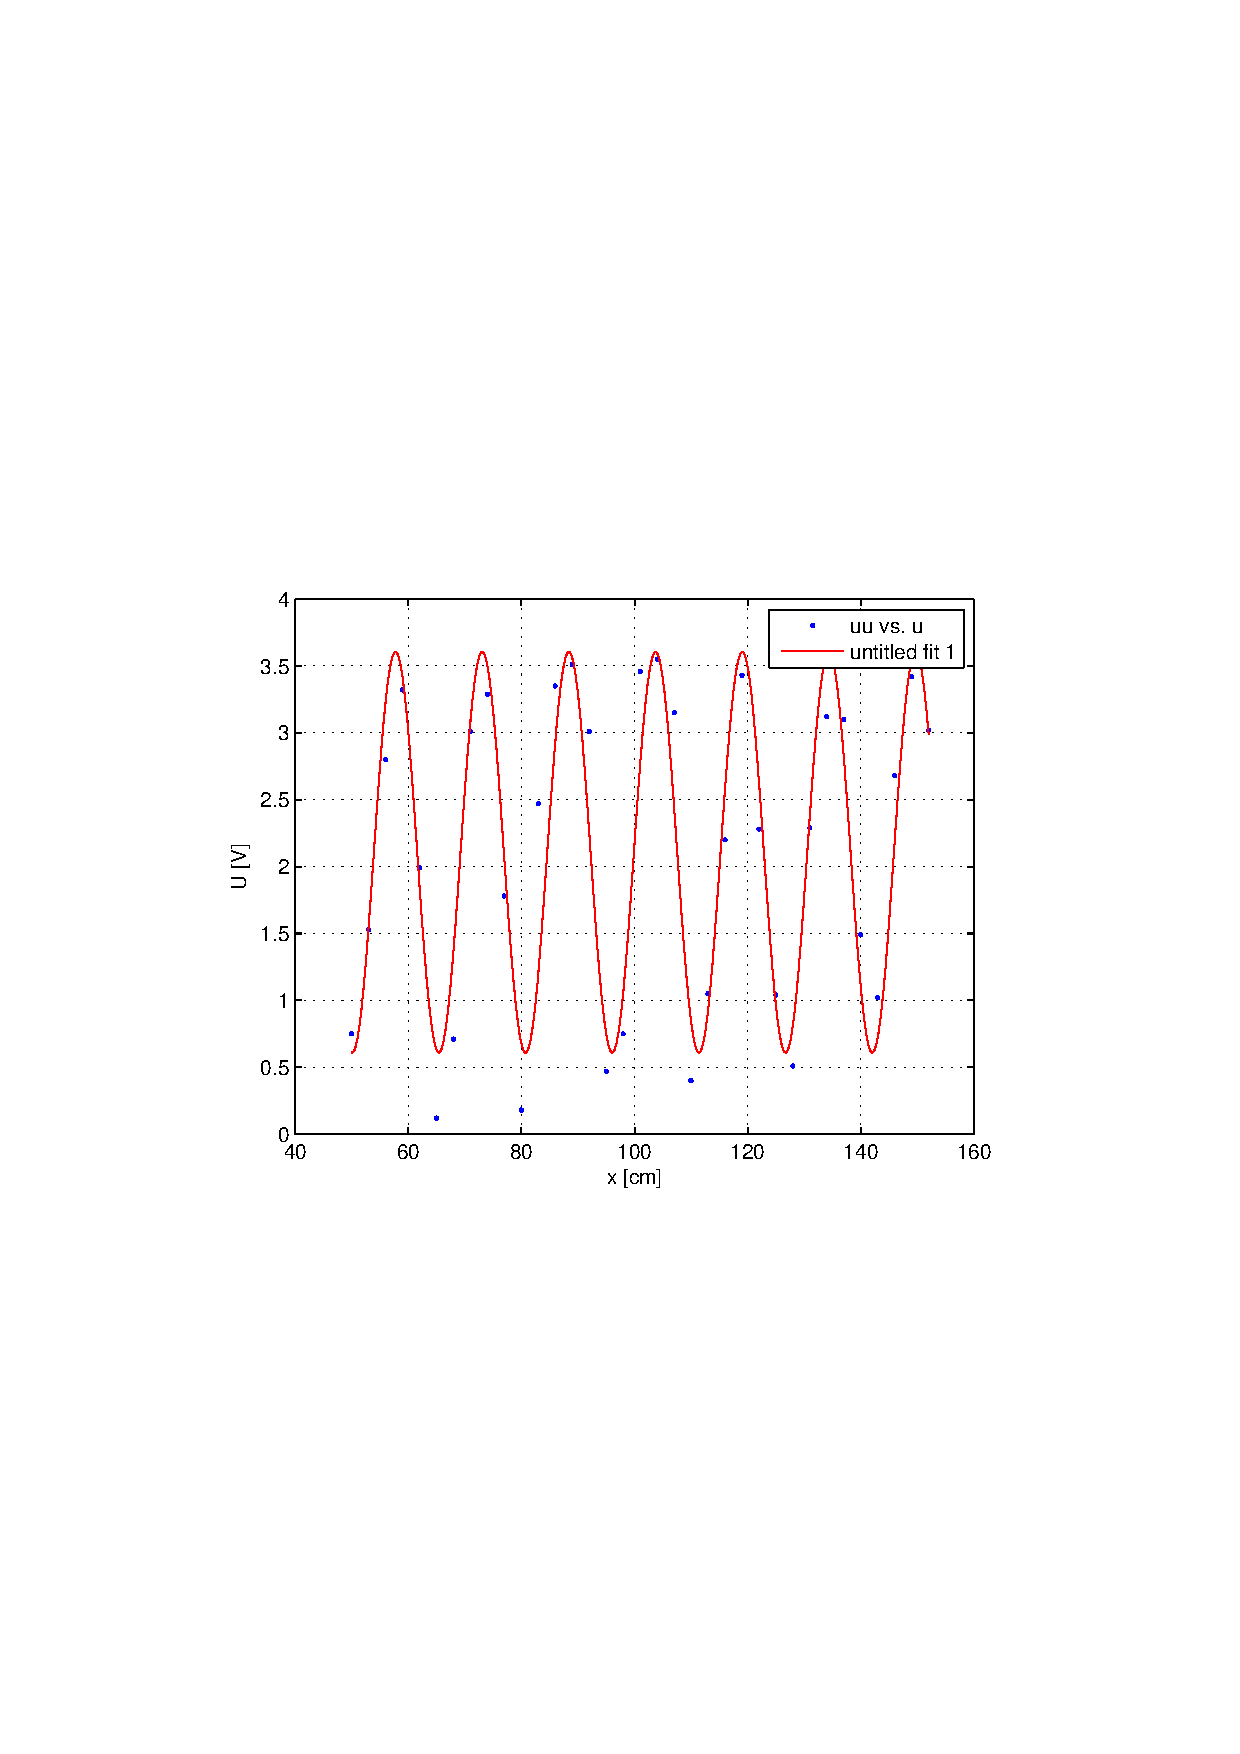
\includegraphics[width=\linewidth]{../gnuplot/3_stoj.pdf}
	    \vspace*{-2cm}
		\caption{Graf závislosti napětí $U$ na vzdálenosti sondy od odrazné kovové desky podél osy $z$. Naměřené hodnoty jsou proloženy funkcí $U(z) = A sin(\omega z+\varphi)+U_0$ a z parametru $\omega$ je pak dopočítána vlnová délka $\lambda$ i s chybou (\ref{eq:chyba_neprime_mereni}).  }
		\label{fig:g_stoj}
	\end{center}
	\end{figure}				
	
	\begin{figure}[h!]
	\begin{center}
	    \vspace*{-1cm}
		\includegraphics[width=\linewidth]{../gnuplot/4_ohyb.pdf}
	    \vspace*{-2cm}
		\caption{Graf závislosti napětí $U$ na poloze sondy před zářičem v příčném směru při proměřování ohybu na hraně. (Kolem hodnoty $x=10$ mm je patrná chybná hodnota.) }
		\label{fig:g_ohyb}
	\end{center}
	\end{figure}			
	
	\begin{figure}[h!]
	\begin{center}
	    \vspace*{-1cm}
		\includegraphics[width=\linewidth]{../gnuplot/4_difrakce.pdf}
	    \vspace*{-2cm}
		\caption{Graf závislosti napětí $U$ na úhlu sondy vzhledem ke štěrbině (dle Obr.~\ref{fig:ohyb_na_sterbine}) při měření difrakce na štěrbině o dvou šířkách. Proložením dvou píků pomocí (\ref{eq:gauss}) z měření pro $D=60$ mm pak byla pomocí (\ref{eq:difrakce}) určena vlnová délka $\lambda$ záření i s chybou (\ref{eq:chyba_neprime_mereni}). }
		\label{fig:g_difrakce}
	\end{center}
	\end{figure}
	
	\begin{figure}[h!]
	\begin{center}
	    \vspace*{-1cm}
		\includegraphics[width=\linewidth]{../gnuplot/4_prekazka.pdf}
	    \vspace*{-2cm}
		\caption{Graf závislosti napětí $U$ na poloze sondy před zářičem v příčném směru při proměřování ohybu na překážce konečných rozměrů ($D=60$ mm). }
		\label{fig:g_prekazka}
	\end{center}
	\end{figure}			
	
	\begin{figure}[h!]
	\begin{center}
	    \vspace*{-1cm}
		\includegraphics[width=\linewidth]{../gnuplot/5_vedeni.pdf}
	    \vspace*{-2cm}
		\caption{Graf závislosti napětí $U$ na poloze sondy podél Lecherova vedení při proměřování stojaté vlny v něm. Naměřené hodnoty jsou proloženy funkcí $U(z) = A sin(\omega z+\varphi)+U_0$ a z parametru $\omega$ je pak dopočítána vlnová délka $\lambda$ i s chybou (\ref{eq:chyba_neprime_mereni}).  }
		\label{fig:g_vedeni}
	\end{center}
	\end{figure}		


\clearpage
\subsection{Schémata}
	\begin{figure}[h!]
	\centering
	\begin{minipage}{.55\textwidth}
	  \centering
				\includegraphics[width=9cm]{att/gunnuv_oscilator_sonda.pdf}
				\caption{Gunnův oscilátor a sonda elektrického pole\newline (převzato z  \cite{bib:zadani}).}
				\label{fig:gunnuv_oscilator_sonda}
	\end{minipage}%
	\hfill
	\begin{minipage}{.35\textwidth}
	  \centering
				\includegraphics[width=5cm]{att/zdroj_napeti_se_zesilovacem.jpg}
				\caption{Zdroj napětí se zesilovačem (převzato z  \cite{bib:zadani}).}
				\label{fig:zdroj_napeti_se_zesilovacem}
	\end{minipage}
	\end{figure}
	
	\begin{figure}[h!]
	\centering
	\begin{minipage}{.40\textwidth}
	  \centering
				\includegraphics[width=7cm]{att/vychozi_nastaveni.jpg}
				\caption{Výchozí nastavení experimentu\newline (převzato z  \cite{bib:zadani}).}
				\label{fig:vychozi_nastaveni}
	\end{minipage}%
	\hfill
	\begin{minipage}{.50\textwidth}
	  \centering
			\includegraphics[width=8cm]{att/soustava_souradnic.jpg}
			\caption{Soustava souřadnic před zářičem (převzato z  \cite{bib:zadani}).}
			\label{fig:soustava_souradnic}
	\end{minipage}
	\end{figure}
	
	\begin{figure}[h!]
	\centering
	\begin{minipage}{.55\textwidth}
	  \centering
			\includegraphics[width=9cm]{att/polarizace_malus.pdf}
			\caption{Ověření Malusova zákona (převzato z  \cite{bib:zadani}).}
			\label{fig:polarizace_malus}
	\end{minipage}%
	\hfill
	\begin{minipage}{.35\textwidth}
	  \centering
			\includegraphics[width=6cm]{att/index_lomu_desky.jpg}
			\caption{Určení indexu lomu dielektrické desky (převzato z  \cite{bib:zadani}).}
			\label{fig:index_lomu_desky}
	\end{minipage}
	\end{figure}	
	
	\begin{figure}[h!]
	\centering
	\begin{minipage}{.50\textwidth}
	  \centering
			\includegraphics[width=8cm]{att/ohyb_na_hrane.jpg}
			\caption{Nastavení experimentu pro ohyb na hraně (převzato z  \cite{bib:zadani}). }
			\label{fig:ohyb_na_hrane}
	\end{minipage}%
	\hfill
	\begin{minipage}{.40\textwidth}
	  \centering
			\includegraphics[width=7cm]{att/ohyb_na_sterbine.jpg}
			\caption{Nastavení aparatury pro ohyb na štěrbině (převzato z  \cite{bib:zadani}).}
			\label{fig:ohyb_na_sterbine}
	\end{minipage}
	\end{figure}	
	
	\begin{figure}[h!]
	\centering
	\begin{minipage}{.45\textwidth}
	  \centering
			\includegraphics[width=7cm]{att/ohyb_na_prekazce.jpg}
			\caption{Nastavení aparatury pro ohyb překážce konečných rozměrů (převzato z  \cite{bib:zadani}).}
			\label{fig:ohyb_na_prekazce}
	\end{minipage}%
	\hfill
	\begin{minipage}{.45\textwidth}
	  \centering
			\includegraphics[width=7cm]{att/zakon_lomu.jpg}
			\caption{Nastavení experimentu pro ověření zákona lomu (převzato z  \cite{bib:zadani}).}
			\label{fig:zakon_lomu}
	\end{minipage}
	\end{figure}	
	
	\begin{figure}[h!]
	\centering
	\begin{minipage}{.55\textwidth}
	  \centering
			\includegraphics[width=9cm]{att/fokusace_cockou.jpg}
			\caption{Fokusace vlnění čočkou (převzato z  \cite{bib:zadani}). }
			\label{fig:fokusace_cockou}
	\end{minipage}
	\hfill
	\begin{minipage}{.35\textwidth}
	  \centering
			\includegraphics[width=6cm]{att/vlnovod.jpg}
			\caption{Zapojení vlnovodu\newline (převzato z  \cite{bib:zadani}). }
			\label{fig:vlnovod}
	\end{minipage}
	\end{figure}		

	\begin{figure}[h]
	\centering
			\includegraphics[width=13cm]{att/lecherovo_vedeni.jpg}
			\caption{Experiment s Lecherovým vedením (převzato z  \cite{bib:zadani}). }
			\label{fig:lecherovo_vlneni}
	\end{figure}	
	
%\clearpage
% --- Konec dokumentu --------------------------------------------------


\end{document}

